\documentclass{article}

\def \lastexercisenumber{10}

% Hier befinden sich Pakete, die wir beinahe immer benutzen ...

\usepackage[utf8]{inputenc}

% Sprach-Paket:
\usepackage[ngerman]{babel}

% damit's nicht so, wie beim Grill aussieht:
\usepackage{fullpage}

% Mathematik:
\usepackage{amsmath, amssymb, amsfonts, amsthm}
\usepackage{bbm}
\usepackage{mathtools, mathdots}

% Makros mit mehereren Default-Argumenten:
\usepackage{twoopt}

% Anführungszeichen (Makro \Quote{}):
\usepackage{babel}

% if's für Makros:
\usepackage{xifthen}
\usepackage{etoolbox}

% tikz ist kein Zeichenprogramm (doch!):
\usepackage{tikz}

% bessere Aufzählungen:
\usepackage{enumitem}

% (bessere) Umgebung für Bilder:
\usepackage{graphicx, subfig, float}

% Umgebung für Code:
\usepackage{listings}

% Farben:
\usepackage{xcolor}

% Umgebung für "plain text":
\usepackage{verbatim}

% Umgebung für mehrerer Spalten:
\usepackage{multicol}

% "nette" Brüche
\usepackage{nicefrac}

% Spaltentypen verschiedener Dicke
\usepackage{tabularx}
\usepackage{makecell}

% Für Vektoren
\usepackage{esvect}

% (Web-)Links
\usepackage{hyperref}

% Zitieren & Literatur-Verzeichnis
\usepackage[style = authoryear]{biblatex}
\usepackage{csquotes}

% so ähnlich wie mathbb
%\usepackage{mathds}

% Keine Ahnung, was das macht ...
\usepackage{booktabs}
\usepackage{ngerman}
\usepackage{placeins}

% special letters:

\newcommand{\N}{\mathbb{N}}
\newcommand{\Z}{\mathbb{Z}}
\newcommand{\Q}{\mathbb{Q}}
\newcommand{\R}{\mathbb{R}}
\newcommand{\C}{\mathbb{C}}
\newcommand{\K}{\mathbb{K}}
\newcommand{\T}{\mathbb{T}}
\newcommand{\E}{\mathbb{E}}
\newcommand{\V}{\mathbb{V}}
\renewcommand{\S}{\mathbb{S}}
\renewcommand{\P}{\mathbb{P}}
\newcommand{\1}{\mathbbm{1}}

% quantors:

\newcommand{\Forall}{\forall \,}
\newcommand{\Exists}{\exists \,}
\newcommand{\ExistsOnlyOne}{\exists! \,}
\newcommand{\nExists}{\nexists \,}
\newcommand{\ForAlmostAll}{\forall^\infty \,}

% MISC symbols:

\newcommand{\landau}{{\scriptstyle \mathcal{O}}}
\newcommand{\Landau}{\mathcal{O}}


\newcommand{\eps}{\mathrm{eps}}

% graphics in a box:

\newcommandtwoopt
{\includegraphicsboxed}[3][][]
{
  \begin{figure}[!h]
    \begin{boxedin}
      \ifthenelse{\isempty{#1}}
      {
        \begin{center}
          \includegraphics[width = 0.75 \textwidth]{#3}
          \label{fig:#2}
        \end{center}
      }{
        \begin{center}
          \includegraphics[width = 0.75 \textwidth]{#3}
          \caption{#1}
          \label{fig:#2}
        \end{center}
      }
    \end{boxedin}
  \end{figure}
}

% braces:

\newcommand{\pbraces}[1]{{\left  ( #1 \right  )}}
\newcommand{\bbraces}[1]{{\left  [ #1 \right  ]}}
\newcommand{\Bbraces}[1]{{\left \{ #1 \right \}}}
\newcommand{\vbraces}[1]{{\left  | #1 \right  |}}
\newcommand{\Vbraces}[1]{{\left \| #1 \right \|}}
\newcommand{\abraces}[1]{{\left \langle #1 \right \rangle}}
\newcommand{\round}[1]{\bbraces{#1}}

\newcommand
{\floorbraces}[1]
{{\left \lfloor #1 \right \rfloor}}

\newcommand
{\ceilbraces} [1]
{{\left \lceil  #1 \right \rceil }}

% special functions:

\newcommand{\norm}  [2][]{\Vbraces{#2}_{#1}}
\newcommand{\diam}  [2][]{\mathrm{diam}_{#1} \: #2}
\newcommand{\diag}  [1]{\mathrm{diag} \: #1}
\newcommand{\dist}  [1]{\mathrm{dist} \: #1}
\newcommand{\mean}  [1]{\mathrm{mean} \: #1}
\newcommand{\erf}   [1]{\mathrm{erf} \: #1}
\newcommand{\id}    [1]{\mathrm{id} \: #1}
\newcommand{\sgn}   [1]{\mathrm{sgn} \: #1}
\newcommand{\supp}  [1]{\mathrm{supp} \: #1}
\newcommand{\arsinh}[1]{\mathrm{arsinh} \: #1}
\newcommand{\arcosh}[1]{\mathrm{arcosh} \: #1}
\newcommand{\artanh}[1]{\mathrm{artanh} \: #1}
\newcommand{\card}  [1]{\mathrm{card} \: #1}
\newcommand{\Span}  [1]{\mathrm{span} \: #1}
\newcommand{\Aut}   [1]{\mathrm{Aut} \: #1}
\newcommand{\End}   [1]{\mathrm{End} \: #1}
\newcommand{\ggT}   [1]{\mathrm{ggT} \: #1}
\newcommand{\kgV}   [1]{\mathrm{kgV} \: #1}
\newcommand{\ord}   [1]{\mathrm{ord} \: #1}
\newcommand{\grad}  [1]{\mathrm{grad} \: #1}
\newcommand{\ran}   [1]{\mathrm{ran} \: #1}
\newcommand{\graph} [1]{\mathrm{graph} \: #1}
\newcommand{\Inv}   [1]{\mathrm{Inv} \: #1}
\newcommand{\pv}    [1]{\mathrm{pv} \: #1}
\newcommand{\GL}    [1]{\mathrm{GL} \: #1}
\newcommand{\Mod}{\mathrm{Mod} \:}
\newcommand{\Th}{\mathrm{Th} \:}
\newcommand{\Char}{\mathrm{char}}
\newcommand{\At}{\mathrm{At}}
\newcommand{\Ob}{\mathrm{Ob}}
\newcommand{\Hom}{\mathrm{Hom}}
\newcommand{\orthogonal}[3][]{#2 ~\bot_{#1}~ #3}
\newcommand{\Rang}{\mathrm{Rang}}
\newcommand{\NIL}{\mathrm{NIL}}
\newcommand{\Res}{\mathrm{Res}}
\newcommand{\lxor}{\dot \lor}
\newcommand{\Div}{\mathrm{div} \:}
\newcommand{\meas}{\mathrm{meas} \:}

% fractions:

\newcommand{\Frac}[2]{\frac{1}{#1} \pbraces{#2}}
\newcommand{\nfrac}[2]{\nicefrac{#1}{#2}}

% derivatives & integrals:

\newcommandtwoopt
{\Int}[4][][]
{\int_{#1}^{#2} #3 ~\mathrm{d} #4}

\newcommandtwoopt
{\derivative}[3][][]
{
  \frac
  {\mathrm{d}^{#1} #2}
  {\mathrm{d} #3^{#1}}
}

\newcommandtwoopt
{\pderivative}[3][][]
{
  \frac
  {\partial^{#1} #2}
  {\partial #3^{#1}}
}

\newcommand
{\primeprime}
{{\prime \prime}}

\newcommand
{\primeprimeprime}
{{\prime \prime \prime}}

% Text:

\newcommand{\Quote}[1]{\glqq #1\grqq{}}
\newcommand{\Text}[1]{{\text{#1}}}
\newcommand{\fastueberall}{\text{f.ü.}}
\newcommand{\fastsicher}{\text{f.s.}}

% -------------------------------- %
% amsthm-stuff:

\theoremstyle{definition}

% numbered theorems
\newtheorem{theorem}{Satz}
\newtheorem{lemma}{Lemma}
\newtheorem{corollary}{Korollar}
\newtheorem{proposition}{Proposition}
\newtheorem{remark}{Bemerkung}
\newtheorem{definition}{Definition}
\newtheorem{example}{Beispiel}

% unnumbered theorems
\newtheorem*{theorem*}{Satz}
\newtheorem*{lemma*}{Lemma}
\newtheorem*{corollary*}{Korollar}
\newtheorem*{proposition*}{Proposition}
\newtheorem*{remark*}{Bemerkung}
\newtheorem*{definition*}{Definition}
\newtheorem*{example*}{Beispiel}

% Please define this stuff in project ("main.tex"):

% \def \lastexercisenumber {...}
% This will be 0 by default

% \setcounter{section}{...}
% This will be 0 by default
% and hence, completely ignored

\ifnum \thesection = 0
{\newtheorem{exercise}{Aufgabe}}
\else
{\newtheorem{exercise}{Aufgabe}[section]}
\fi

\ifdef
{\lastexercisenumber}
{\setcounter{exercise}{\lastexercisenumber}}

\newcommand{\solution}
{
    \renewcommand{\proofname}{Lösung}
    \renewcommand{\qedsymbol}{}
    \proof
}

\renewcommand{\proofname}{Beweis}

% -------------------------------- %
% environment zum einkasteln:

% dickere vertical lines
\newcolumntype
{x}
[1]
{!{\centering\arraybackslash\vrule width #1}}

% environment selbst (the big cheese)
\newenvironment
{boxedin}
{
  \begin{tabular}
  {
    x{1 pt}
    p{\textwidth}
    x{1 pt}
  }
  \Xhline
  {2 \arrayrulewidth}
}
{
  \\
  \Xhline{2 \arrayrulewidth}
  \end{tabular}
}

% -------------------------------- %
% MISC "Ein-Deutschungen"

\renewcommand
{\figurename}
{Abbildung}

\renewcommand
{\tablename}
{Tabelle}

% -------------------------------- %


\addbibresource{../../../Fundament-LaTeX/references.bib}

\graphicspath{{../../../Fundament-LaTeX/images/}}

\parindent 0pt

\title
{
  Numerik von Partiellen Differentialgleichungen: stationäre Probleme \\
  \vspace{4pt}
  \normalsize
  \textit{3. Übung am 11.11.2020}
}
\author
{
  Richard Weiss
  \and
  Florian Schager
  \and
  Christian Sallinger
  \and
  Fabian Zehetgruber
  \and
  Paul Winkler
  \and
  Christian Göth
}
\date{}

\begin{document}

\maketitle

% --------------------------------------------------------------------------------

\begin{exercise}

\phantom{}

\begin{enumerate}[label = \textbf{\alph*)}]

  \item Sei $(T_j)_{j \in \N} \subset \R^2$ eine Folge von nicht-degenerierten Dreiecken.
  Zeigen Sie, dass die shape regularity Konstanten $\sigma(T_j) = h_{T_j} / \rho_{T_j}$ genau dann gegen unendlich divergieren wenn der kleinste Winkel in $T_j$ gegen Null geht.

  \item Eine alternative Definition der shape regularity Konstante ist gegeben durch $\tilde{\sigma}(T) := h_T / r_t$, wobei

  \begin{align*}
    r_T := \max
    \Bbraces
    {
      \text{diam}(B):
      B ~\text{ein Kreis enthalten in}~ T
    }.
  \end{align*}

  Wie hängen $\sigma(T)$ und $\tilde{\sigma}(T)$ zusammen?

\end{enumerate}
  
\end{exercise}
  
  % --------------------------------------------------------------------------------
  
  \begin{solution}

  \phantom{}

  \begin{figure}[h!]
    \centering
    \begin{tikzpicture}[scale=1.25]

      \coordinate [label = left:        $A$] (A) at (0, 0);
      \coordinate [label = below right: $B$] (B) at (8, 0);
      \coordinate [label = above:       $C$] (C) at (2, 4);
      \draw
        (A) -- node [below]       {$c$}
        (B) -- node [above right] {$a$}
        (C) -- node [above left]  {$b$}
        cycle;

        \coordinate (M) at (2, 0);
        \draw (C) -- node [right] {$h$} (M);

        \draw (1, 0) node [above] {$c_A$};
        \draw (5, 0) node [above] {$c_B$};

        \draw (0.5, 0) arc (0:64:0.5);
        \draw (0.25, 0.15) node {$\alpha$};

        \draw (7, 0) arc (180:146:1);
        \draw (7.25, 0.2) node {$\beta$};

        \draw (2, 3) arc (270:243.5:1);
        \draw (2, 3) arc (270:326:1);
        \draw (2.35, 3.4) node {$\gamma$};

        \draw (2.25, 0) arc (0:90:0.25);
        \draw (2.1, 0.1) node {$\cdot$};

      \end{tikzpicture}
      \caption{Dreieck $T$}
      \label{fig:dreieck}
  \end{figure}
  
  \begin{enumerate}[label = \textbf{\alph*)}]
  
    \item Sei $T$ ein Dreieck.
    Man betrachte die Skizze aus Abbildung \ref{fig:dreieck}.
    Der $\sin$-Satz besagt Folgendes.

    \begin{align*}
      \frac{a}{\sin \alpha}
      =
      \frac{b}{\sin \beta}
      =
      \frac{c}{\sin \gamma}
    \end{align*}
  
    $\arcsin$ steigt monoton und $c \geq a, b$.

    \begin{align*}
      \implies
      \gamma
      =
      \arcsin \frac{c \sin \gamma}{c}
      \geq
      \begin{cases}
        \arcsin \frac{a \sin \gamma}{c} = \alpha \\
        \arcsin \frac{b \sin \gamma}{c} = \beta
      \end{cases}
    \end{align*}
    
    Also ist $\gamma$ der größte Winkel ($\to$ uninteressant).
  
    \begin{align*}
      \implies
      \sigma(T)
      =
      \frac{c}{h}
      =
      \frac{c_A + c_B}{h}
      =
      \frac{c_A}{h} + \frac{c_B}{h}
      =
      \frac{1}{\tan \alpha} + \frac{1}{\tan \beta}
    \end{align*}
  
    Daraus folgt die Behauptung.
  
    \item Sei $r$ der Inkreis-Radius und $d = 2r$ der Inkreis-Durchmesser.
    Wikipedia kennt folgende Formel.
  
    \begin{align*}
      r = \frac{2 |T|}{a + b + c} = \frac{ch}{a + b + c}
    \end{align*}
  
    \begin{align*}
      \implies
      \sigma(T)
      =
      \frac{c}{h}
      \leq
      \frac{c}{d}
      =
      \tilde{\sigma}(T)
      =
      \frac{c}{d}
      =
      \frac{c}
      {
        2 \frac{ch}{a + b + c}
      }
      =
      \frac{a + b + c}{2h}
      \leq
      \frac{3c}{2h}
      =
      \frac{3}{2} \sigma(T)
    \end{align*}
  
  \end{enumerate}
  
  \end{solution}
  
  % --------------------------------------------------------------------------------
  
% --------------------------------------------------------------------------------

\begin{exercise}

Sei $P_p:= \mathcal{L} \Bbraces{x^i y^j: i, j \geq 0 \land i+j \leq p}$ für $p \in \N$ der Raum der Polynome vom maximalen Grad $p$.

\begin{enumerate}[label = \textbf{\alph*)}]

  \item Geben Sie eine Basis von $P_0$ an.

  \item Zeigen Sie, dass die Funktionen

  \begin{align}
    \lambda_1(x, y) := 1-x-y, 
    \quad
    \lambda_2(x, y) := x, 
    \quad
    \lambda_3(x, y) := y
  \end{align}

  eine Basis des $P_1$ bilden.

  \item Zeigen Sie, dass die Funktionen $\lambda_1, \lambda_2, \lambda_3, \lambda_1 \lambda_2, \lambda_1 \lambda_3, \lambda_2\lambda_3$ eine Basis des $P_2$ bilden.

  \item Zeigen Sie, dass eine Basis des $P_p$ für $p \geq 3$ aus folgenden Funktionen gebildet werden kann:

  \begin{enumerate}[label = (\roman*)]
    \item $(x, y) \mapsto \lambda_j(x, y)$ mit $1 \leq j \leq 3$
    \item $(x, y) \mapsto p_{jk}(x, y)\lambda_j(x, y)\lambda_k(x, y)$ mit $1 \leq k < j \leq 3$ und
    \item $(x, y) \mapsto p_{123}(x, y) \prod_{j=1}^3 \lambda_j(x, y)$ und $p_{123} \in P_{p-3}$
  \end{enumerate}

  Die folgenden Einschränkungen der Polynome $p_{jk}$ sind dabei jeweils eindimensionale Polynome vom maximalen Grad $p-2: \xi \mapsto p_{12}(\xi, 0), \xi \mapsto p_{13}(0, \xi)$ und $\xi \mapsto p_{23}(\xi, 1-\xi)$.

  \item Erklären Sie andhand des Referenzdreiecks mit den Eckpunkten $(0, 0)$, $(1, 0)$ und $(0, 1)$ die Bedeutung dieser Aufgabe auf eine Erweiterung von Proposition $3.1$ auf Polynomräume höheren Grades.

\end{enumerate}

\end{exercise}

% --------------------------------------------------------------------------------

\begin{solution}

\begin{align*}
  \lambda_1(x, y) & = 1 - x - y \\
  \lambda_2(x, y) & = x \\
  \lambda_3(x, y) & = y \\
  (\lambda_1 \lambda_2)(x, y) & = x - x^2 - xy \\
  (\lambda_2 \lambda_3)(x, y) & = xy \\
  (\lambda_3 \lambda_1)(x, y) & = y - xy - y^2 \\
  (\lambda_1 \lambda_2 \lambda_3)(x, y) & = xy - x^2 y - x y^2
\end{align*}

\begin{align*}
  B_p(x, y) := (1, x, y, x^2, xy, y^2, \dots, x^p, \dots, y^p)
\end{align*}

\begin{enumerate}[label = \textbf{\alph*)}]

  \item

  \begin{align*}
    \Lambda_0 := (1)
  \end{align*}

  \begin{align*}
    \implies
    B_0(x, y) = \Lambda_0(x, y)
  \end{align*}
  
  \item

  \begin{align*}
    \Lambda_1
    :=
    \begin{pmatrix}
      \lambda_1 \\
      \lambda_2 \\
      \lambda_3
    \end{pmatrix}
  \end{align*}

  \begin{align*}
    \implies
    \underbrace
    {
      \begin{pmatrix}
        1 & -1 & -1 \\
          &  1 &    \\
          &    &  1
      \end{pmatrix}
    }_{
      =: T_1 \in \GL(6, \R)
    }
    B_1(x, y)
    =
    \Lambda_1(x, y)
  \end{align*}

  \item

  \begin{align*}
    \Lambda_2
    :=
    \begin{pmatrix}
      \Lambda_1 \\
      \lambda_1 \lambda_2 \\
      \lambda_2 \lambda_3 \\
      \lambda_3 \lambda_1
    \end{pmatrix}
  \end{align*}

  \begin{align*}
    \implies
    \underbrace
    {
      \pbraces
      {
        \begin{array}{ccc|ccc}
          &     &    &    & & \\
          & T_1 &    &    & & \\
          &     &    &    & & \\
          \hline
          & 1   &    & -1 & -1 & \\
          &     &    &    &  1 & \\
          &     &  1 & -1 &    & -1
        \end{array}
      }
    }_{
      =: T_2 \in \GL(6, \R)
    }
    B_2(x, y)
    =
    \Lambda_2(x, y)
  \end{align*}

  \item Wir definieren unsere Basis rekursiv.
  
  RA($p = 3$):

  \begin{align*}
    \Lambda_3(x, y)
    :=
    \begin{pmatrix}
      \Lambda_2(x, y) \\
      x \lambda_1(x, y) \lambda_2(x, y) \\
      x \lambda_2(x, y) \lambda_3(x, y) \\
      y \lambda_3(x, y) \lambda_1(x, y) \\
      x \lambda_3(x, y) \lambda_1(x, y)
    \end{pmatrix}
    =
    \begin{pmatrix}
      \Lambda_2 \\
      p_{12} \lambda_1 \lambda_2 \\
      p_{23} \lambda_2 \lambda_3 \\
      p_{31} \lambda_3 \lambda_1 \\
      \lambda_1 \lambda_2 \lambda_3
    \end{pmatrix}
    (x, y)
  \end{align*}

  $\Lambda_3$ ist linear unabhängig, weil $\Lambda_2$ es ist und jede Funktion $f$, ist zu $\id \cdot f$.
  Wir müssen die Transformationsmatrix also nicht einmal explizit hinschreiben. \\

  RS($p \mapsto p+1$):

  (i)-(iii) bedeuten hier, dass man $p_{12}$ mit $x$ und $p_{21}$ mit $y$ sowie $p_{23}, p_{123}$ entweder mit $x$ oder $y$ multiplizieren darf.
  Die Polynome werden dann (i)-(iii) im $p+1$ setting erfüllen.

  Seien $\Lambda_{p-1}$ und $\Lambda_p$ Basen von $P_p$ bzw. $P_{p-1} \subset P_p \subset P_{p+1}$.
  Wir ergänzen $\Lambda_p$ zu einer Basis $\Lambda_{p+1}$ von $P_{p+1}$, die (i)-(iii) für $p+1$ erfüllt.

  Die Elemente aus $\Lambda_p \setminus \Lambda_{p-1}$ (und $\Lambda_{p-1}$) haben folgende Form.

  \begin{align*}
    p_{12} \lambda_1 \lambda_2,
    \quad
    p_{23} \lambda_2 \lambda_3,
    \quad
    p_{31} \lambda_3 \lambda_1,
    \quad
    p_{123} \lambda_1 \lambda_2 \lambda_3,
    \quad
    (\text{und}~ \lambda_1, \lambda_2, \lambda_3)
  \end{align*}

  Polynome 1. und 3. Form multiplizieren wir mit $x$ bzw $y$;
  bei den anderen dürfen wir es uns jeweils aussuche, z.B. immer $x$.
  Wir erhalten $|\Lambda_p \setminus \Lambda_{p-1}| = p$ neue Polynome.
  Für das $(p+1)$-te Polynom nehmen wir die 2. oder 4. Form mal $y$.
  
  \begin{align*}
    \begin{Bmatrix}
      p_{12} \lambda_1 \lambda_2 \\
      p_{23} \lambda_2 \lambda_3 \\
      p_{31} \lambda_3 \lambda_1 \\
      p_{123} \lambda_1 \lambda_2 \lambda_3
    \end{Bmatrix}
    \mapsto
    \begin{Bmatrix}
      x \, p_{12} \lambda_1 \lambda_2 \\
      x \, p_{23} \lambda_2 \lambda_3 \\
      y \, p_{31} \lambda_3 \lambda_1 \\
      x \, p_{123} \lambda_1 \lambda_2 \lambda_3 \\
      y \, p_{123} \lambda_1 \lambda_2 \lambda_3
    \end{Bmatrix}
    \mapsto
    \begin{Bmatrix}
      x x \, p_{12} \lambda_1 \lambda_2 \\
      x x \, p_{23} \lambda_2 \lambda_3 \\
      y y \, p_{31} \lambda_3 \lambda_1 \\
      x x \, p_{123} \lambda_1 \lambda_2 \lambda_3 \\
      x y \, p_{123} \lambda_1 \lambda_2 \lambda_3 \\
      y y \, p_{123} \lambda_1 \lambda_2 \lambda_3
    \end{Bmatrix}
    \mapsto
    \begin{Bmatrix}
      x x x \, p_{12} \lambda_1 \lambda_2 \\
      x x x \, p_{23} \lambda_2 \lambda_3 \\
      y y y \, p_{31} \lambda_3 \lambda_1 \\
      x x x \, p_{123} \lambda_1 \lambda_2 \lambda_3 \\
      x x y \, p_{123} \lambda_1 \lambda_2 \lambda_3 \\
      x y y \, p_{123} \lambda_1 \lambda_2 \lambda_3 \\
      y y y \, p_{123} \lambda_1 \lambda_2 \lambda_3
    \end{Bmatrix}
    \mapsto \dots
  \end{align*}
  
  \item

  \begin{figure}[h!]
    \centering
    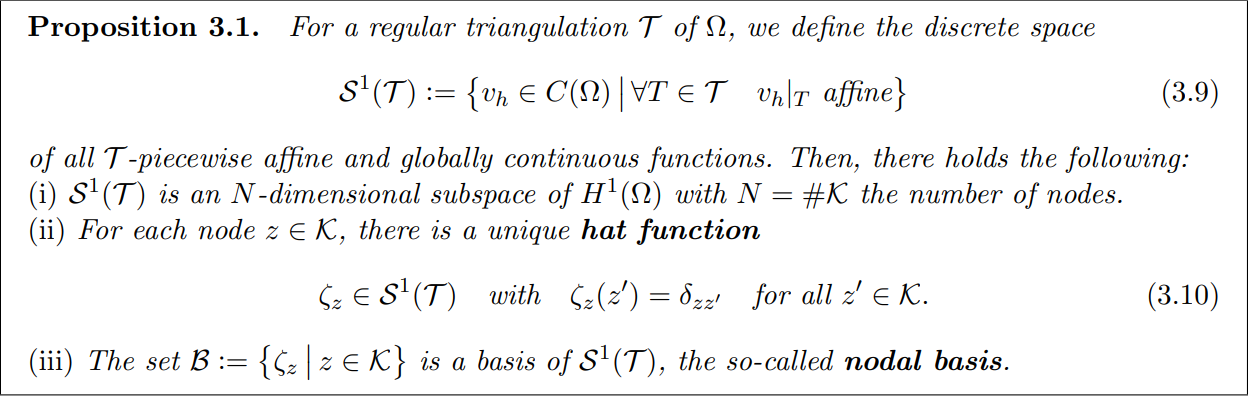
\includegraphics
    [width = 0.75 \textwidth]
    {NumPDEs/NumPDEs - Proposition 3.1.png}
    \caption{\cite{NumPDEs}}
  \end{figure}

  Die Basisvektoren aus $\Lambda_p$ sind nodal, d.h.

  \begin{align*}
    \Forall \lambda \in \Lambda_p,
    \Forall E \in \mathcal{E}_{T_\mathrm{ref}}:
    \lambda(E) \in \Bbraces{0, 1}.
  \end{align*}

  Das sieht man leicht durch Einsetzten der Refernez-Eckpunkte.
  Es sei dabei bemerkt, dass wir nur mit $x$ bzw. $y$ multipliziert haben.

\end{enumerate}

\end{solution}

% --------------------------------------------------------------------------------

% --------------------------------------------------------------------------------

\begin{exercise}

Gegeben sei ein zusammenhängender ungerichteter Graph $G = (V,E)$ mit einer geraden Anzahl an Knoten.
Zeigen Sie, dass es einen (nicht notwendigerweise zusammenhängenden) Untergraph mit
Knotenmenge $V$ gibt (also einen Graph $G^\prime = (V, E^\prime)$ mit $E^\prime \subseteq E$),
in dem alle Knotengrade ungerade sind.

(Hinweis: beweisen Sie die Behauptung für Bäume und begründen Sie, warum diese Annahme reicht.)

\end{exercise}

% --------------------------------------------------------------------------------

\begin{solution}
Der Grad eines Knoten $v \in V$
ist definert als $\grad(x) = |\{\{x,y\}: \{x,y\} \in E\}|$. \\
Wir beweisen die Aussage mit Induktion nach $n := |V|$: \\
Für $n = 2$ gibt es genau eine Kante, welche die beiden Knoten verbindet,
also gilt die Aussage bereits für $E^{\prime} = E$. \\
Induktionsschritt: $n \rightsquigarrow n + 2$: \\
Betrachte einen beliebigen Baum $G$ mit $V = \{x_1,\dots,x_{n+2}\}$.
Nun existiert ein $v \in V$ mit $\grad(v) = 1$ (o.B.d.A. $v = x_{n+2}$).
Nun ist $G_1 = (V_1,E_1)$ mit
\begin{align*}
  V_1 &:= \{x_1,\dots,x_{n+1}\} \\
  E_1 &:= \{\{x,y\} \in E: x,y \in V_1\}
\end{align*}
klarerweise immer noch zyklenfrei und zusammenhängend und wir können
ein weiteres $v \in V_1$ mit $\grad(v) = 1$ (o.B.d.A: $v = x_{n+1}$) finden, sodass
dann $G = (V_2,E_2)$ mit
\begin{align*}
  V_2 &:= \{x_1,\dots,x_{n}\} \\
    E_1 &:= \{\{x,y\} \in E: x,y \in V_2\}
\end{align*}
ein zusammenhängender, zyklenfreier Graph ist, auf den wir die Induktionsvoraussetzung
anwenden können, also erhalten wir $E_2^{\prime} \subseteq E_2$, sodass
für alle $v \in V_2: \grad(v) = 1$. \\
Nun definieren wir $E^{\prime} = E_2^{\prime} \cup \{\{x_n,x_{n+1}\}\}$, welches
die Bedingung dann für alle $v \in V$ erfüllt. \\


Für einen beliebig zusammenhängenden Graphen $G = (V,E)$ mit gerader Knotenanzahl
erinnern wir uns daran, dass
ein Baum genau ein minimal zusammenhängender Graph ist.
Also finden wir in jedem Fall ein $E_1 \subseteq E$, sodass $G_1 = (V,E_1)$
ein Baum ist und wir das soeben gezeigte anwenden können.
\end{solution}

% --------------------------------------------------------------------------------

% -------------------------------------------------------------------------------- %

\begin{exercise}

Formulieren und beweisen Sie das Lemma $3.8$ explizit für den Fall $m=2$.

\end{exercise}

% -------------------------------------------------------------------------------- %

\begin{solution}

\begin{figure}[h!]
  \centering
  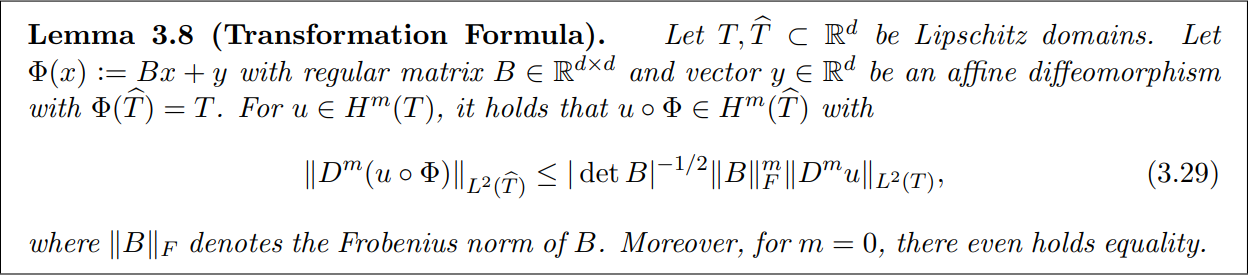
\includegraphics
  [width = 0.75 \textwidth]
  {NumPDEs/NumPDEs - Lemma 3.8 (Transformation Formula).png}
\end{figure}

\begin{align*}
  \Psi:
  C^\infty(\overline T) \to H^2(\hat T):
  u \mapsto u \circ \Phi
\end{align*}

Wir zeigen zuerst die Wohldefiniertheit von $\Psi$ als linearer und
beschränkter Operator, d.h. $\Exists C > 0:$

\begin{align*}
  \norm[H^2(\hat T)]{\Psi u}
  \leq
  C \norm[H^2(T)]{u}.
\end{align*}

Dazu zeigen wir zunächst die Transformationsfomel für $u \in C^{\infty}(\overline{T})$ und $m = 0,1,2$.

\begin{enumerate}[label = \arabic*.]

  \item Abschätzung ($m = 0$):
  Die steht sogar explizit im Skript.

  \begin{align*}
    \implies
    \norm[L^2(T)]{u}^2
    =
    \Int[T]{u^2}{y}
    =
    \Int[\hat T]{(u \circ \Phi)^2 |\det D \Phi|}{x}
    =
    |\det B| \norm[L^2(\hat T)]{u \circ \Phi}^2
  \end{align*}

  \item Abschätzung ($m = 1$):

  \begin{align*}
    \implies
    \partial_j (u \circ \Phi)(x)
    =
    \sum_{n=1}^d
    \partial_n u(\Phi(x)) B_{nj}
  \end{align*}

  Jetzt verwenden wir die Cauchy-Schwarz-Bunjakovski Ungleichung.

  \begin{align*}
    \implies
    |\partial_j (u \circ \Phi)(x)|^2
    & \stackrel
    {
      \mathrm{CSB}
    }
    {\leq}
    \pbraces
    {
      \sum_{n=1}^d
      \partial_n u(\Phi(x))|^2
    }
    \pbraces
    {
      \sum_{n=1}^d
      B_{nj}^2
    }
    =
    |Du(\Phi(x))|^2
    \pbraces
    {
      \sum_{n=1}^d
      B_{nj}^2
    }
    \end{align*}

  Jetzt verwenden wir die Transformationsfomel.

  \begin{align*}
    \implies
    |\det B| \norm[L^2(\hat T)]{D(u \circ \Phi)}^2
    & =
    \Int[\hat T]
    {
      \sum_{j=1}^d
      |\partial_j (u \circ \Phi)(x)|^2
      |\det D \Phi(x)|
    }{x} \\
    & \leq
    \Int[\hat T]
    {
      \sum_{j=1}^d
      |Du(\Phi(x))|^2
      \pbraces
      {
        \sum_{n=1}^d
        B_{nj}^2
      }
      |\det D \Phi(x)|
    }{x} \\
    & =
    \sum_{j=1}^d
    \pbraces
    {
      \sum_{n=1}^d
      B_{nj}^2
    }
    \Int[\hat T]
    {
      |Du(\Phi(x))|^2
      |\det D \Phi(x)|
      }{x} \\
    & \stackrel
    {
      \mathrm{TRAFO}
    }{=}
    \sum_{j=1}^d
    \pbraces
    {
      \sum_{n=1}^d
      B_{nj}^2
    }
    \Int[T]
    {
      |Du(x)|^2
    }{x} \\
    & =
    \norm[F]{B}^2 \norm[L^2(T)]{Du}^2
  \end{align*}

  \item Abschätzung ($m = 2$):

  \begin{align*}
    \implies
    D(u \circ \Phi) = Du(\Phi(x))D\Phi(x) = Du(\Phi(x))B
  \end{align*}

  \begin{align*}
    \implies
    \partial_k \partial_j (u \circ \Phi)(x)
    &=
    \partial_k \pbraces
    {
      \sum_{n=1}^d
      \partial_n u(\Phi(x)) B_{nj}
    } \\
    &=
    \sum_{n=1}^d
    B_{nj} \partial_k (\partial_n u(\Phi(x)))
    =
    \sum_{n=1}^d
    \sum_{m=1}^d
    \partial_m \partial_n u(\Phi(x)) B_{nj} B_{mk}
  \end{align*}

  Jetzt verwenden wir Cauchy-Schwarz-Bunjakovski.

  \begin{align*}
    \implies
    |\partial_k \partial_j (u \circ \Phi)(x)|^2
    &\stackrel
    {
      \mathrm{CSB}
    }
    {\leq}
    \pbraces
    {
      \sum_{n,m=1}^d
      |\partial_m \partial_n u(\Phi(x))|^2
    }
    \pbraces
    {
      \sum_{n,m=1}^d |B_{nj} B_{mk}|^2
    } \\
    &=
    |D^2 u(\Phi(x))|^2
    \pbraces
    {
      \sum_{n=1}^d
      B_{nj}^2
    }
    \pbraces
    {
      \sum_{m=1}^d
      B_{mk}^2
    }
  \end{align*}

  Jetzt verwenden wir die Transformationsfomel.

  \begin{align*}
    \implies
    |\det B| \norm[L^2(\hat T)]{D^2(u\circ\Phi)}^2
    & =
    \Int[\hat T]
    {
      \sum_{j=1}^d
      \sum_{k=1}^d
      |\partial_k \partial_j (u \circ \Phi)(x)|^2
      |\det D\Phi(x)|
    }{x} \\
    & \leq
    \Int[\hat T]
    {
      \sum_{j=1}^d
      \sum_{k=1}^d
      |D^2 u (\Phi(x))|^2
      \pbraces
      {
        \sum_{n=1}^d
        B_{nj}^2
      }
      \pbraces
      {
        \sum_{m=1}^d
        B_{mk}^2
      }
      |\det D \Phi(x)|
    }{x} \\
    & =
    \sum_{j=1}^d
    \sum_{k=1}^d
    \pbraces
    {
      \sum_{n=1}^d
      B_{nj}^2
    }
    \pbraces
    {
      \sum_{m=1}^d
      B_{mk}^2
    }
    \Int[\hat T]
    {
      |D^2 u (\Phi(x))|^2
      |\det D \Phi(x)|
    }{x} \\
    & \stackrel
    {
      \mathrm{TRAFO}
    }{=}
    \sum_{j=1}^d
    \sum_{k=1}^d
    \pbraces
    {
      \sum_{n=1}^d
      B_{nj}^2
    }
    \pbraces
    {
      \sum_{m=1}^d
      B_{mk}^2
    }
    \Int[T]{|D^2 u(x)|^2}{x} \\
    & =
    \pbraces
    {
      \sum_{j=1}^d
      \sum_{n=1}^d
      B_{nj}^2
    }
    \pbraces
    {
      \sum_{k=1}^d
      \sum_{m=1}^d
      B_{mk}^2
    }
    \norm[L^2(T)]{D^2 u}^2 \\
    & =
    \norm[F]{B}^4 \norm[L^2(T)]{D^2 u}^2.
  \end{align*}

\end{enumerate}

Mit diesen Abschätzungen bekommen wir die Stetigkeit von $\Psi$, d.h. $\Exists C > 0:$

\begin{multline*}
  \norm[H^2(\hat T)]{\Psi u}
  =
  \norm[H^2(\hat T)]{u \circ \Phi}
  =
  \norm[L^2(\hat T)]{u \circ \Phi}^2
  +
  \norm[L^2(\hat T)]{D (u \circ \Phi)}^2
  +
  \norm[L^2(\hat T)]{D^2 (u \circ \Phi)}^2 \\
  \leq
  |\det B|^{-1/2}
  \pbraces
  {
    \norm[L^2(T)]{u}^2
    +
    \norm[F]{B}^2
    \norm[L^2(T)]{Du}^2
    +
    \norm[F]{B}^4
    \norm[L^2(T)]{D^2 u}^2
  }
  \leq
  C^2 \norm[H^2(T)]{u}^2.
\end{multline*}

Als nächstes erweitern wir das Resultat mit Dichtheitsargumenten auf den ganzen $H^2(T)$.

$C^{\infty}(\overline{T})$ liegt ja dicht in $H^2(T)$.
$\Phi$ kann somit (eindeutig) stetig auf dem ganzen Raum $H^2(T)$ fortgesetzt werden
(sogar normerhaltend).

Wir wollen nun zeigen, dass für $\Forall u \in H^2(T):$

\begin{align*}
  \Psi u = u \circ \Phi.
\end{align*}

Sei dazu $u \in H^2(T)$ und $(u_n)_{n \in \N} \subset C^{\infty}(\overline{T})$ mit

\begin{align*}
  u_n \xrightarrow[n \to \infty]{H^2(T)} u.
\end{align*}

Aufgrund der $\norm[H^2]{\cdot}$-Stetigkeit von $\Psi$, erhalten wir damit auch

\begin{align*}
  \implies
  u_n \circ \Phi = \Psi(u_n) \xrightarrow[n \to \infty]{H^2(T)} \Psi u.
\end{align*}

Weil $\norm[L^2]{\cdot} \leq \norm[H^2]{\cdot}$, erhalten wir für $(u_n)_{n \in \N}$ auch $L^2(T)$-Konvergenz.

\begin{align*}
  \implies
  u_n \xrightarrow[n \to \infty]{L^2(T)} u
\end{align*}

Weil $u$ messbar ist, können wir die Transformationsformel darauf anwenden.
Die 1. Abschätzung ($m = 0$) liefert uns also

\begin{align*}
  u_n \circ \Phi \xrightarrow[n \to \infty]{L^2(\hat T)} u \circ \Phi.
\end{align*}

Weil Grenzwerte eindeutig sind, folgt unsere Behauptung.

\begin{align*}
  \implies
  u \circ \Phi = \Psi u
\end{align*}

Nun ist jede Norm $\norm{\cdot}$ in sich selbst stetig ($\norm{\cdot}$-stetig), und

\begin{align*}
  u_n \xrightarrow[n \to \infty]{H^2(T)} u,
  \quad
  u_n \circ \Phi \xrightarrow[n \to \infty]{H^2(\hat T)} u \circ \Phi.
\end{align*}

Ähnlich wie vorher gilt $\norm[L^2]{D^2 (\cdot)} \leq \norm[H^2]{\cdot}$.

\begin{align*}
  \implies
  D^2 u_n \xrightarrow[n \to \infty]{L^2(T)} D^2 u,
  \quad
  D^2 (u_n \circ \Phi) \xrightarrow[n \to \infty]{L^2(\hat T)} D^2 (u \circ \Phi)
\end{align*}


\begin{align*}
  \implies
  \norm[L^2(\hat T)]{D^2(u\circ\Phi)}
  &=
  \lim_{n \to \infty}
  \norm[L^2(\hat T)]{D^2(u_n\circ\Phi)} \\
  &\leq
  \lim_{n \to \infty}
  |\det B|^{-1/2}
  \norm[F]{B}^2
  \norm[L^2(T)]{D^2 u_n}
  =
  |\det B|^{-1/2}
  \norm[F]{B}^2
  \norm[L^2(T)]{D^2 u}
\end{align*}

\end{solution}

% -------------------------------------------------------------------------------- %

\begin{exercise}

Hier könnte Ihre Werbung stehen!

\begin{itemize}
  \item[(a)] Definieren Sie Konvergenz im Maß, fast überall, fast gleichmäßig, fast überall gleichmäßig.
  \item[(b)] $(X_n)$ sei eine Folge von unabhängigen Zufallsvariablen. Zeigen Sie, dass genau dann fast sicher
  \begin{align*}
    \lim_{n \to \infty} X_n = 0
  \end{align*}
  gilt, wenn für jedes $\epsilon > 0$
  \begin{align*}
    \sum_{n \in \N} \P(|X_n| > \epsilon) < \infty.
  \end{align*}
\end{itemize}

\end{exercise}

% --------------------------------------------------------------------------------

\begin{solution}

(a) Siehe Aufgabe 1. \\

(b) Hier könnte Ihre Werbung stehen!

\begin{itemize}

  \item[\Quote{$\Rightarrow$}:] Angenommen, $\Exists \epsilon > 0:$
  \begin{align*}
    \sum_{n \in \N} \P(|X_n| > \epsilon) = \infty,
  \end{align*}
  dann gilt laut dem \Quote{zweiten Lemma von Borel-Cantelli}, dass
  \begin{align*}
    \P(\limsup_{n \in \N} [|X_n| > \epsilon]) = 1.
  \end{align*}
  $\limsup_{n \in \N} [|X_n| > \epsilon]$ ist dabei die Menge aller Punkte, die in unendlich vielen $[|X_n| > \epsilon]$ enthalten ist.

  \item[\Quote{$\Leftarrow$}:]
  $1 - \P(|X_n| \leq \epsilon)
  =
  \P(|X_n| > \epsilon)
  \xrightarrow[n \to \infty]{} 0$

\end{itemize}

\end{solution}


\printbibliography

\end{document}
